\chapter{Understanding Local Computation Overhead in NOC-NOC}
\section{Overview}

Guided by \textbf{NOC-NOC}, \cite{multazzu2023nocs} designed two algorithms for two concurrency control levels: Read Atomicy and Transactional Causal Consistency. Interested readers can refer to \cite{multazzu2023nocs} for more details. Essentially, the client maintains version vectors to view the database states.  It also holds two views of the database states: the global safe vector version and the local safe vector version. By maintaining these metadata, the client could check the incoming transactions version and its local versions to maintain safety properties within one round of communication, thus satisfying the \textbf{O} property: \textit{One Round of Communication}. However, this is not without its penalty. It has to recursively scan all the dual states in the database to find the most recent version before being committed.  In contrast, the Eiger \cite{lloyd2013stronger} and the Eiger-Port \cite{lu2020performance} algorithms may incur additional network round trips, but require less local computation overhead. 


Although there are many technical details behind these algorithms, there is one \textit{fundamental} thinking.  To successfully commit a distributed transaction, we have to pay some cost. This cost could be paid either via network communication or via local computation on the client side or on the server side. The actual transaction performance depends on the performance of the hardware (local computation CPU, network bandwidth) and the distribution of the cost each hardware has to pay. It is a common belief that in the distributed transaction protocol, we should minimize the network round trip as much as possible. However, this is usually at the cost of increasing local computation. If we increase the local computation burden and the local CPU becomes over-utilized, but the network becomes under-utilized, this may lead to suboptimal performance.

\textbf{NOC-NOC} principles and algorithms guided by these principles seek to minimize the network round trip and increase local computation overhead compared with algorithms such as Eiger \cite{lloyd2013stronger} and Eiger-PORT \cite{lu2020performance}. Although \cite{multazzu2023nocs} has shown that \textbf{NOC-NOC} is generally considered better than these two algorithms, in this chapter, we try to test these algorithms under certain corner cases and try to understand the local computation overhead between these algorithms and design principles.
\section{Experimental Setup}
\paragraph{Code Base.} For Eiger \cite{lloyd2013stronger} and Eiger-PORT \cite{lu2020performance}, we used its original code base. For \textbf{RA-NOC2} and \textbf{Eiger-NOC2}, we also used its original code base. 

\paragraph{Workload.} We used the YCSB benchmark \cite{cooper2010benchmarking}. YCSB is a key-value benchmark that Yahoo collects for many usages, including testing the performance of key-value stores, different concurrency control protocols. We mainly used workload A for testing. Workload A is a read-dominant workload, but the read-write ratio could be tuned for different purposes. Unless otherwise stated, we use the default parameter settings in YCSB.

\paragraph{Setup.} We used the CloudLab \cite{duplyakin2019design} as the testbed.  We used the XL170 node on the Utah cluster. The machine has 2 10-Core, 3.4 GHz, Xeon E5-2640 v4 CPUs and the network bandwidth is 10Gbps. 

\paragraph{Measurements.} 
In each of the experiments, we measure the overall throughput, average latency, and the 99th latency. We run experiments for two different concurrency levels: Read Atomic and Causal Consistency. Unless otherwise stated, we used the default parameters. By default, each transaction contains 8 operations. The default zipfian factor is 0 (uniform distribution). We used 5 servers and 5 clients by default. The value size is 64B and the number of keys is 1K by default. We run the experiment 5 times and take the average.

\section{Experimental Results}
\subsection{Large Transaction Size}
We experiment with different concurrency control algorithms concerning large transaction sizes. The first three figures are at the Read Atomic level. The last three are at the causal consistent level.
 Here are the results. Refer to Figure \ref{fig:1}, Figure \ref{fig:2}, Figure \ref{fig:3}, Figure \ref{fig:4}, Figure \ref{fig:5}, Figure \ref{fig:6}. Results show that NOC2 based algorithms outperform all other baselines under large transaction size.
\begin{figure}
    \centering
    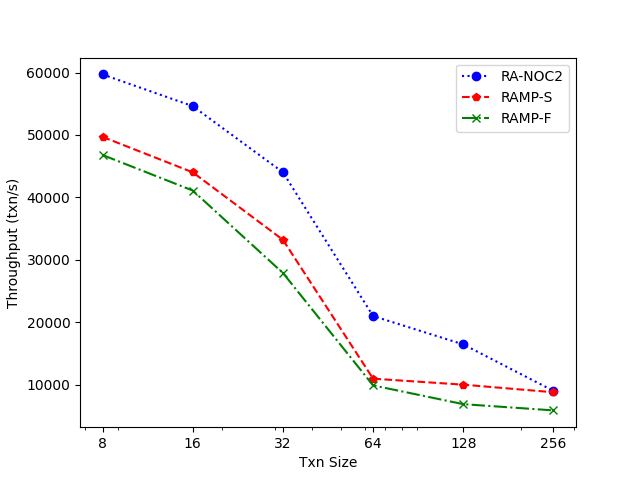
\includegraphics[width=0.8\linewidth]{figure/1-ra-t.png}
    \caption{Throughput Comparison for Three Different Concurrency Control Algorithms under Different Transaction Size in Read Atomicity Level}
    \label{fig:1}
\end{figure}



\begin{figure}
    \centering
    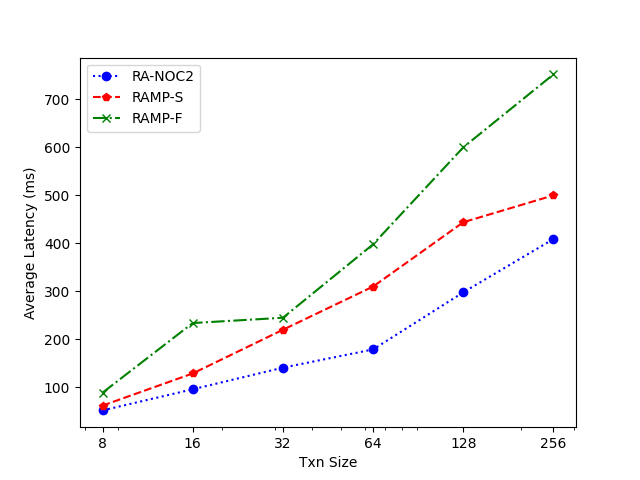
\includegraphics[width=0.8\linewidth]{figure/1-ra-al.png}
    \caption{Average Latency Comparison for Three Different Concurrency Control Algorithms under Different Transaction Size in Read Atomicity Level}
    \label{fig:2}
\end{figure}


\begin{figure}
    \centering
    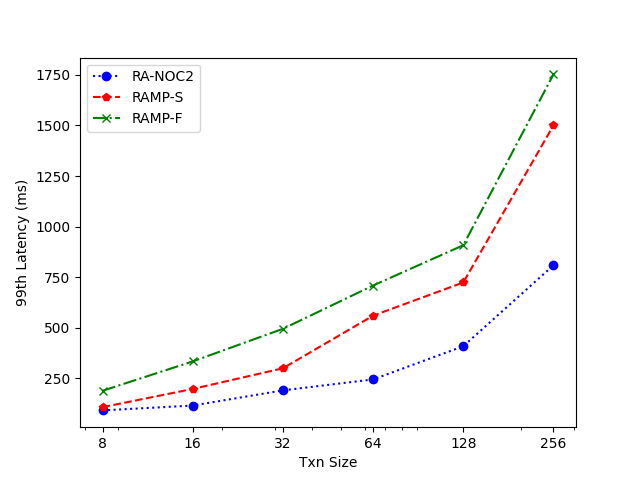
\includegraphics[width=0.8\linewidth]{figure/1-ra-l.png}
    \caption{99th Latency Comparison for Three Different Concurrency Control Algorithms under Different Transaction Size in Read Atomicity Level}
    \label{fig:3}
\end{figure}


\begin{figure}
    \centering
    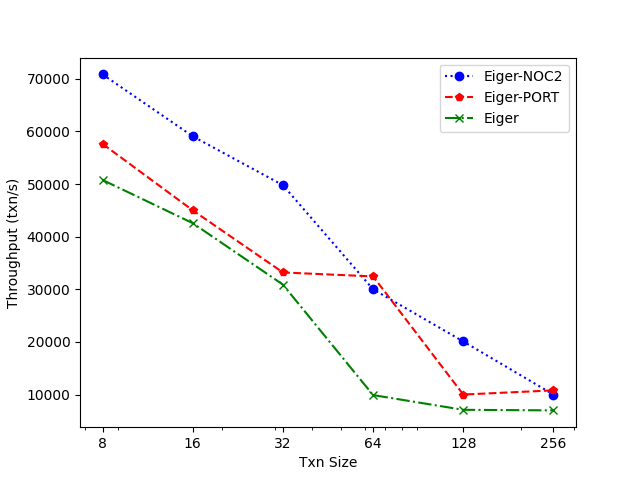
\includegraphics[width=0.8\linewidth]{figure/1-tcc-t.png}
    \caption{Throughput Comparison for Three Different Concurrency Control Algorithms under Different Transaction Size in Causal Consistency Level}
    \label{fig:4}
\end{figure}


\begin{figure}
    \centering
    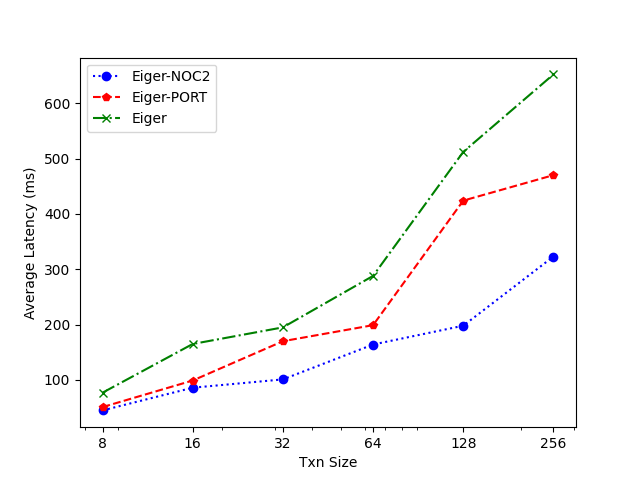
\includegraphics[width=0.8\linewidth]{figure/1-tcc-al.png}
    \caption{Average Latency Comparison for Three Different Concurrency Control Algorithms under Different Transaction Size in Causal Consistency Level}
    \label{fig:5}
\end{figure}


\begin{figure}
    \centering
    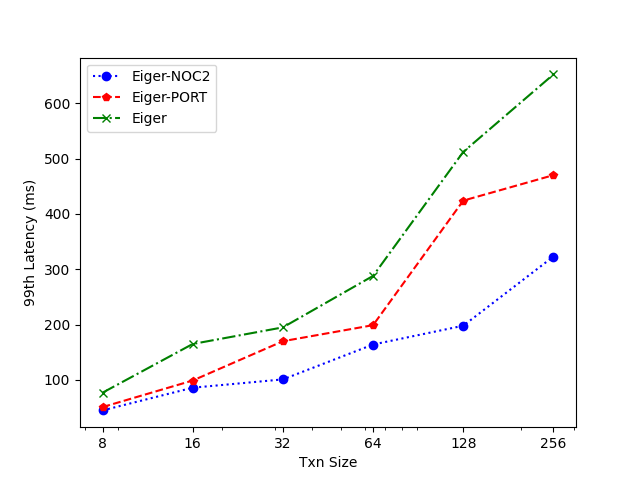
\includegraphics[width=0.8\linewidth]{figure/1-tcc-l.png}
    \caption{99th Latency Comparison for Three Different Concurrency Control Algorithms under Different Transaction Size in Causal Consistency Level}
    \label{fig:6}
\end{figure}

\newpage

\subsection{Large Number of Servers}
We experiment with different concurrency control algorithms concerning large number of servers. The first three figures are at the Read Atomic level. The last three are at the causal consistent level. Here are the results. Refer to Figure ~\ref{fig:7}, Figure ~\ref{fig:8}, Figure ~\ref{fig:9}, Figure \ref{fig:10}, Figure \ref{fig:11}, Figure \ref{fig:12}.  Results show that NOC2 based algorithms outperform all other baselines under different number of servers.


\begin{figure}[H]
    \centering
    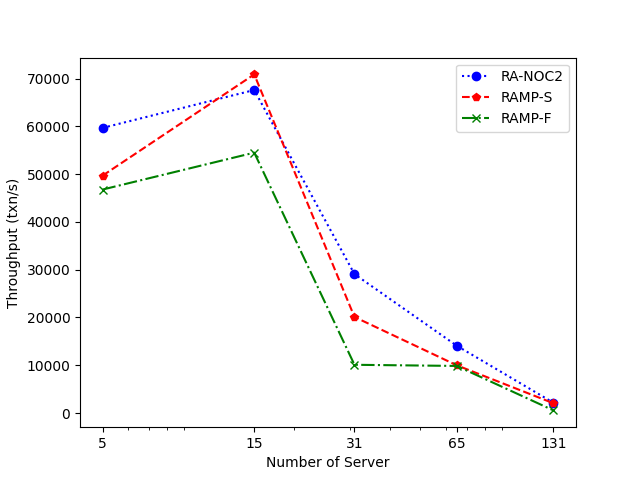
\includegraphics[width=0.8\linewidth]{figure/3-ra-t.png}
    \caption{Throughput Comparison for Three Different Concurrency Control Algorithms under Different Number of Servers in Read Atomicity Level}
    \label{fig:7}
\end{figure}

\begin{figure}[H]
    \centering
    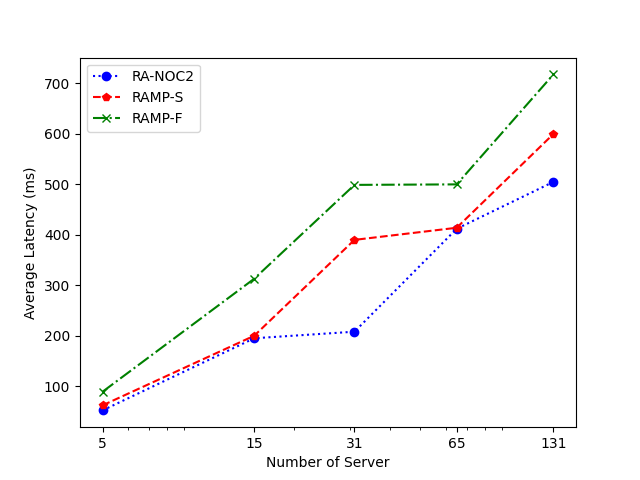
\includegraphics[width=0.8\linewidth]{figure/3-ra-al.png}
    \caption{Average Latency Comparison for Three Different Concurrency Control Algorithms under Different Number of Servers in Read Atomicity Level}
    \label{fig:8}
\end{figure}


\begin{figure}[H]
    \centering
    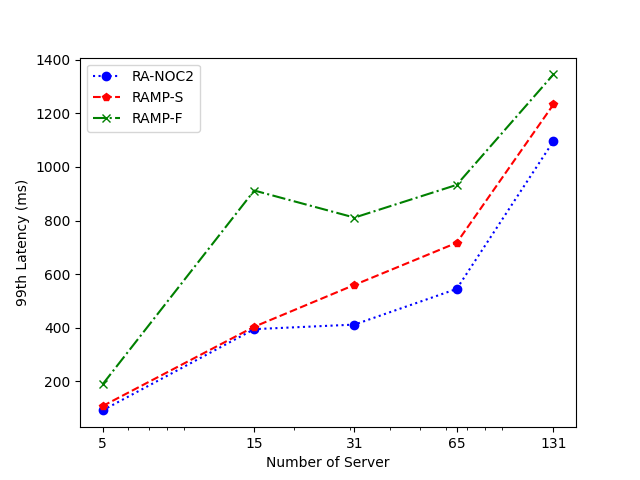
\includegraphics[width=0.8\linewidth]{figure/3-ra-l.png}
    \caption{99th Latency Comparison for Three Different Concurrency Control Algorithms under Different Number of Servers in Read Atomicity Level}
    \label{fig:9}
\end{figure}


\begin{figure}[H]
    \centering
    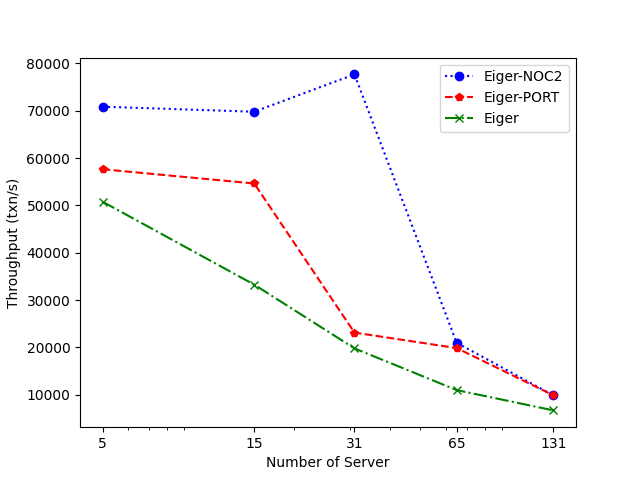
\includegraphics[width=0.8\linewidth]{figure/3-tcc-t.png}
    \caption{Throughput Comparison for Three Different Concurrency Control Algorithms under Different Number of Servers in Causal Consistency Level}
    \label{fig:10}
\end{figure}


\begin{figure}[H]
    \centering
    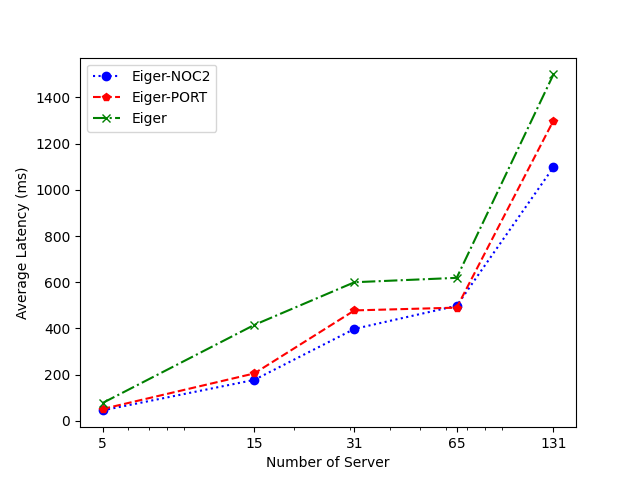
\includegraphics[width=0.8\linewidth]{figure/3-tcc-al.png}
    \caption{Average Latency Comparison for Three Different Concurrency Control Algorithms under Different Number of Servers in Causal Consistency Level}
    \label{fig:11}
\end{figure}


\begin{figure}[H]
    \centering
    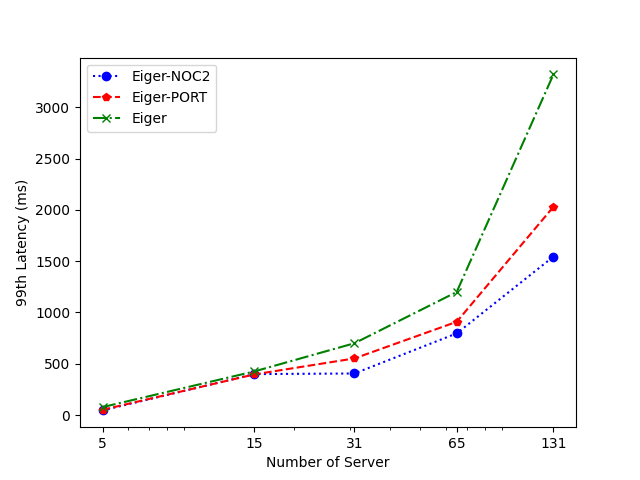
\includegraphics[width=0.8\linewidth]{figure/3-tcc-l.png}
    \caption{99th Latency Comparison for Three Different Concurrency Control Algorithms under Different Number of Servers in Causal Consistency Level}
    \label{fig:12}
\end{figure}


\newpage


\subsection{Large Number of Clients}
We experiment with different concurrency control algorithms concerning large number of clients. The first three figures are at the Read Atomic level. The last three are at the causal consistent level. Here are the results. Refer to Figure ~\ref{fig:13}, Figure ~\ref{fig:14}, Figure ~\ref{fig:15}, Figure \ref{fig:16}, Figure \ref{fig:17}, Figure \ref{fig:18}. Results show that NOC2 based algorithms outperform all other baselines under different number of clients. 



\begin{figure}[H]
    \centering
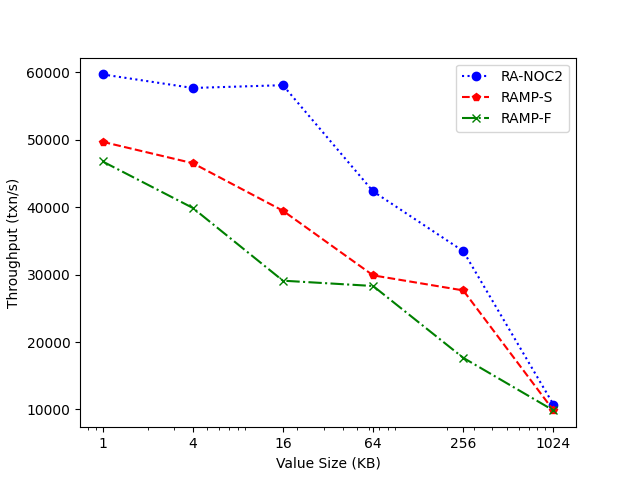
\includegraphics[width=0.8\linewidth]{figure/5-ra-t.png}
    \caption{Throughput Comparison for Three Different Concurrency Control Algorithms under Different Number of Clients in Read Atomicity Level}
    \label{fig:13}
\end{figure}
\begin{figure}[H]
    \centering
    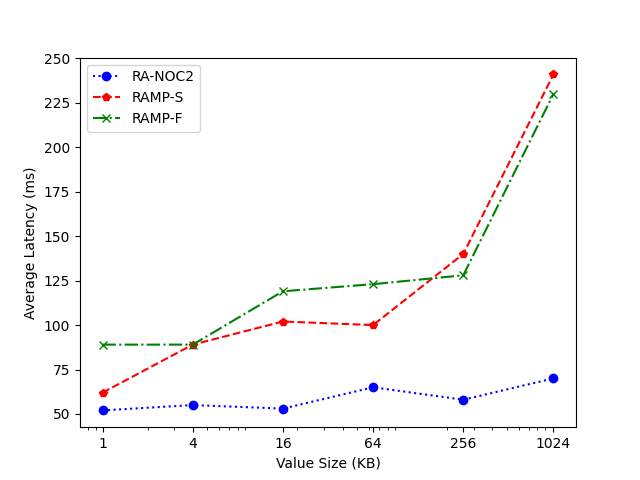
\includegraphics[width=0.8\linewidth]{figure/5-ra-al.png}
    \caption{Average Latency Comparison for Three Different Concurrency Control Algorithms under Different Number of Clients in Read Atomicity Level}
    \label{fig:14}
\end{figure}
\begin{figure}[H]
    \centering
    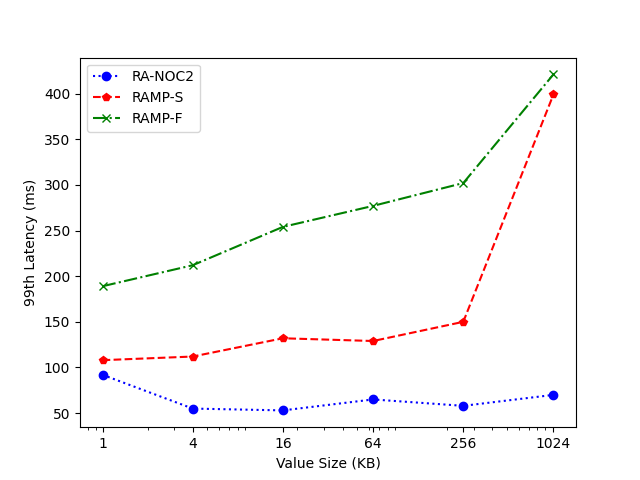
\includegraphics[width=0.8\linewidth]{figure/5-ra-l.png}
    \caption{99th Latency Comparison for Three Different Concurrency Control Algorithms under Different Number of Clients in Read Atomicity Level}
    \label{fig:15}
\end{figure}
\begin{figure}[H]
    \centering
    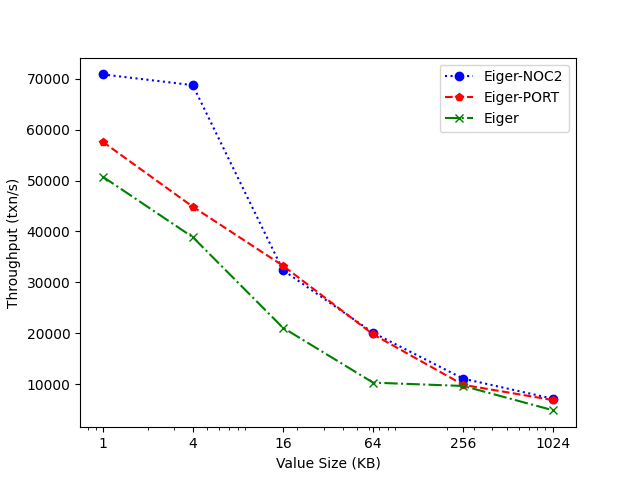
\includegraphics[width=0.8\linewidth]{figure/5-tcc-t.png}
    \caption{Throughput Comparison for Three Different Concurrency Control Algorithms under Different Number of Clients in Causal Consistency Level}
    \label{fig:16}
\end{figure}
\begin{figure}[H]
    \centering
    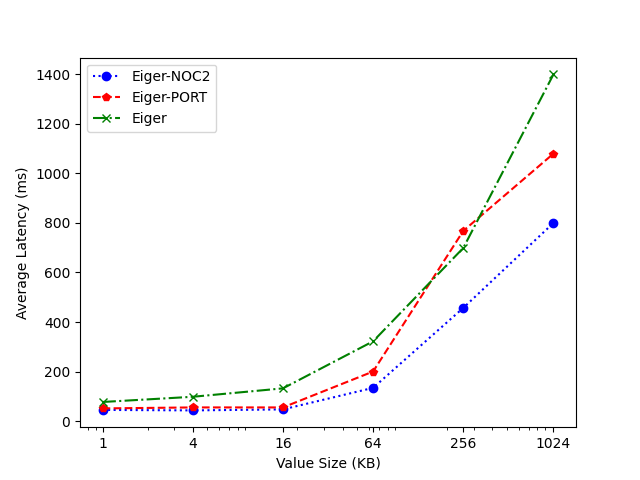
\includegraphics[width=0.8\linewidth]{figure/5-tcc-al.png}
    \caption{Average Latency Comparison for Three Different Concurrency Control Algorithms under Different Number of Clients in Causal Consistency Level}
    \label{fig:17}
\end{figure}
\begin{figure}[H]
    \centering
    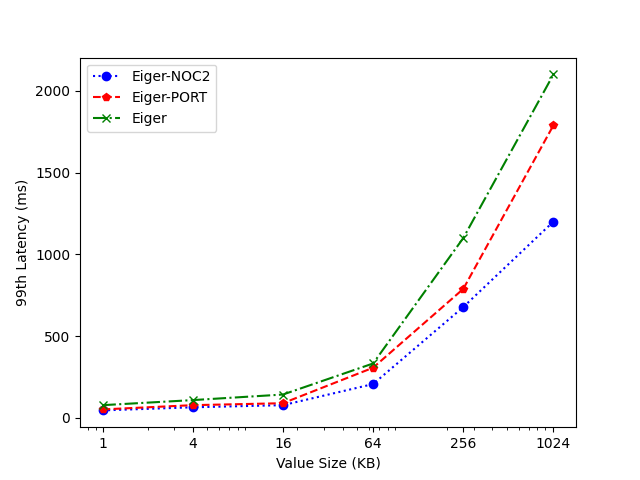
\includegraphics[width=0.8\linewidth]{figure/5-tcc-l.png}
    \caption{99th Latency Comparison for Three Different Concurrency Control Algorithms under Different Number of Clients in Causal Consistency Level}
    \label{fig:18}
\end{figure}

\subsection{Large Value Size}

We experiment with different concurrency control algorithms concerning large value size. The first three figures are at the Read Atomic level. The last three are at the causal consistent level. Here are the results. Refer to Figure ~\ref{fig:19}, Figure ~\ref{fig:20}, Figure ~\ref{fig:21}, Figure \ref{fig:22}, Figure \ref{fig:23}, Figure \ref{fig:24}. 
 Results show that NOC2 based algorithms outperform all other baselines under different value size.
\begin{figure}[H]
    \centering
    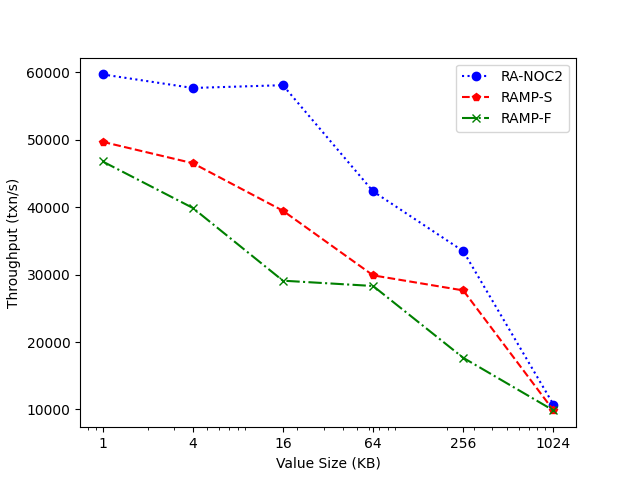
\includegraphics[width=0.8\linewidth]{figure/5-ra-t.png}
    \caption{Throughput Comparison for Three Different Concurrency Control Algorithms under Different Value Size in Read Atomicity Level}
    \label{fig:19}
\end{figure}
\begin{figure}[H]
    \centering
    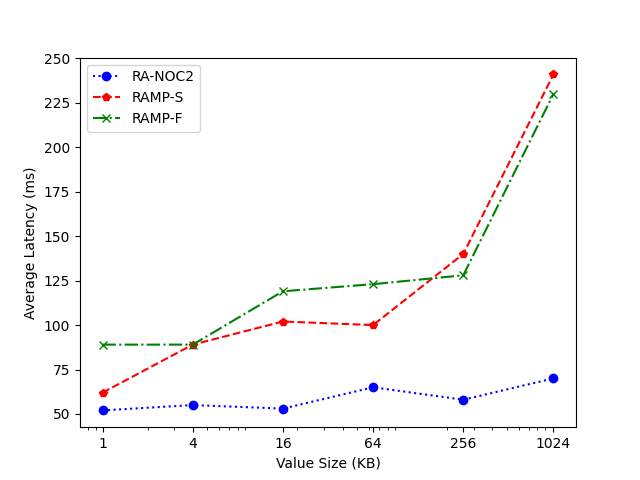
\includegraphics[width=0.8\linewidth]{figure/5-ra-al.png}
    \caption{Average Latency Comparison for Three Different Concurrency Control Algorithms under Different Value Size in Read Atomicity Level}
    \label{fig:20}
\end{figure}
\begin{figure}[H]
    \centering
    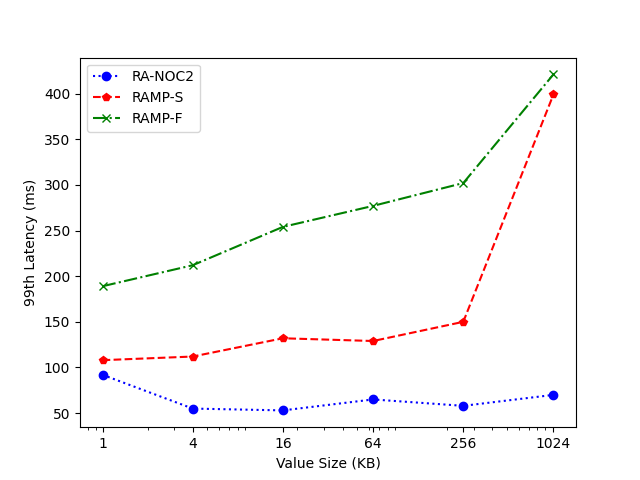
\includegraphics[width=0.8\linewidth]{figure/5-ra-l.png}
    \caption{99th Latency Comparison for Three Different Concurrency Control Algorithms under Different Value Size in Read Atomicity Level}
    \label{fig:21}
\end{figure}
\begin{figure}[H]
    \centering
    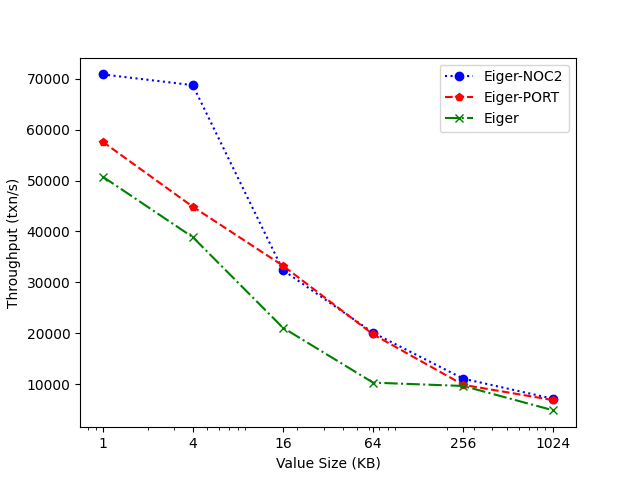
\includegraphics[width=0.8\linewidth]{figure/5-tcc-t.png}
    \caption{Throughput Comparison for Three Different Value Size under Different Number of Clients in Causal Consistency Level}
    \label{fig:22}
\end{figure}
\begin{figure}[H]
    \centering
    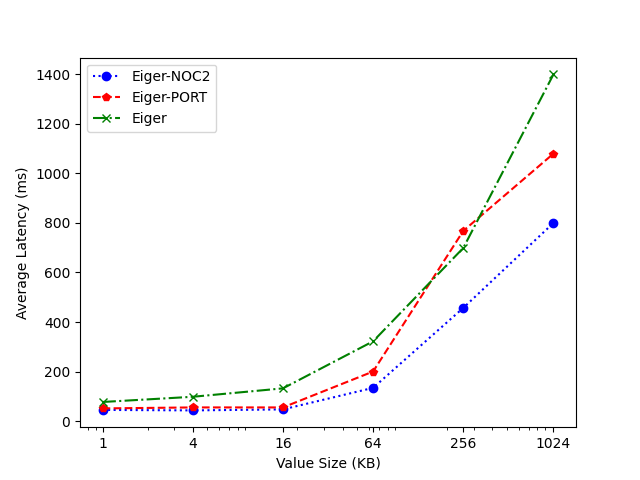
\includegraphics[width=0.8\linewidth]{figure/5-tcc-al.png}
    \caption{Average Latency Comparison for Three Different Concurrency Control Algorithms under Different Value Size in Causal Consistency Level}
    \label{fig:23}
\end{figure}
\begin{figure}[H]
    \centering
    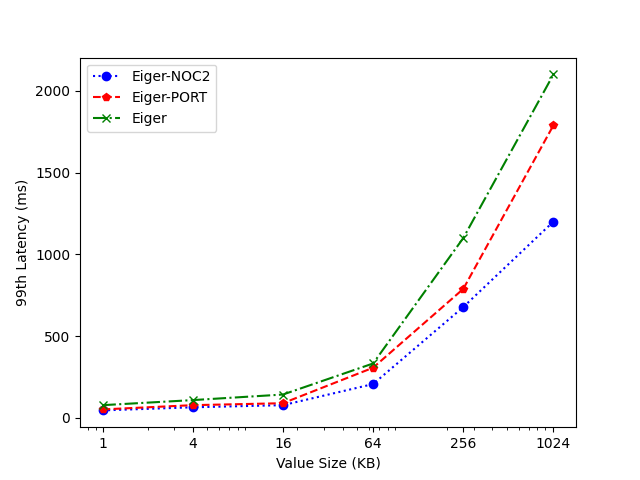
\includegraphics[width=0.8\linewidth]{figure/5-tcc-l.png}
    \caption{99th Latency Comparison for Three Different Concurrency Control Algorithms under Different Value Size in Causal Consistency Level}
    \label{fig:24}
\end{figure}



\subsection{Large Number of Keys}

We experiment with different concurrency control algorithms concerning large number of keys. The first three figures are at the Read Atomic level. The last three are at the causal consistent level. Here are the results. Refer to Figure ~\ref{fig:25}, Figure ~\ref{fig:26}, Figure ~\ref{fig:27}, Figure \ref{fig:28}, Figure \ref{fig:29}, Figure \ref{fig:30}. 

Results show that NOC2 based algorithms outperform all other baselines under large number of keys.
\begin{figure}[H]
    \centering
    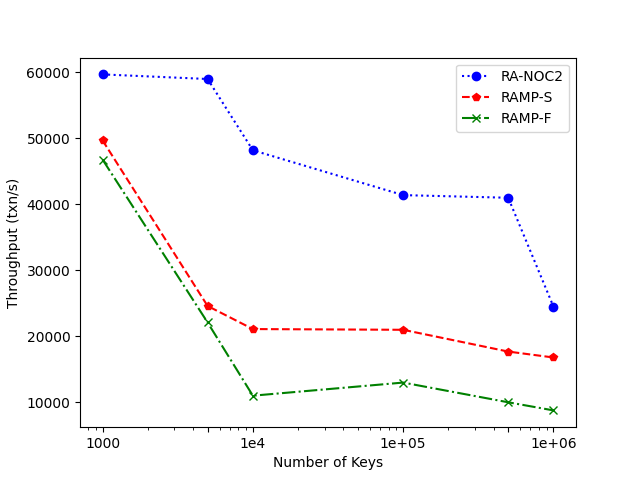
\includegraphics[width=0.8\linewidth]{figure/6-ra-t.png}
    \caption{Throughput Comparison for Three Different Concurrency Control Algorithms under Different Number of Keys in Read Atomicity Level}
    \label{fig:25}
\end{figure}
\begin{figure}[H]
    \centering
    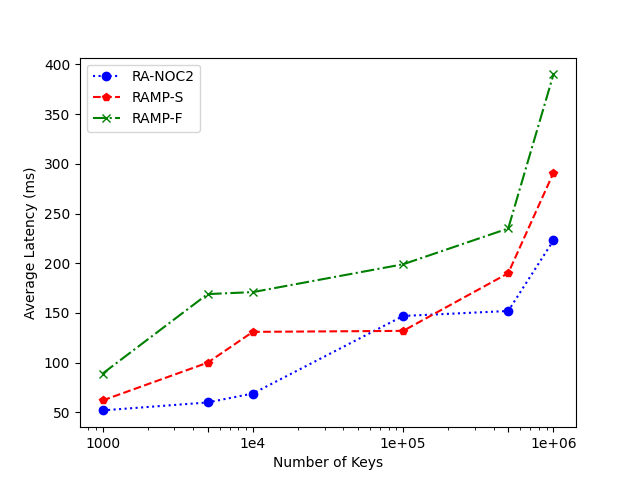
\includegraphics[width=0.8\linewidth]{figure/6-ra-al.png}
    \caption{Average Latency Comparison for Three Different Concurrency Control Algorithms under Different Number of Keys in Read Atomicity Level}
    \label{fig:26}
\end{figure}
\begin{figure}[H]
    \centering
    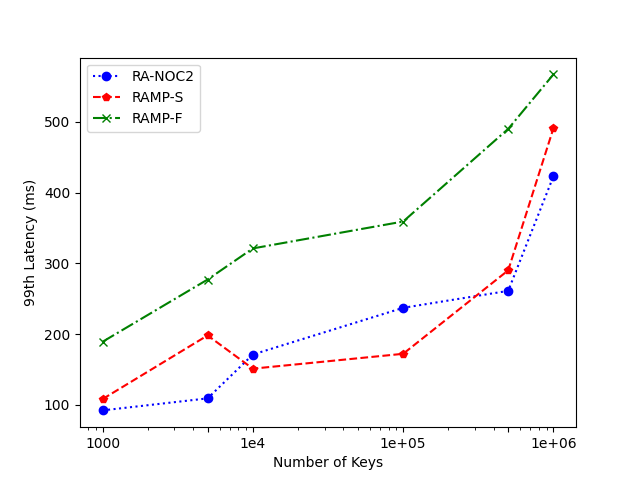
\includegraphics[width=0.8\linewidth]{figure/6-ra-l.png}
    \caption{99th Latency Comparison for Three Different Concurrency Control Algorithms under Different Number of Keys in Read Atomicity Level}
    \label{fig:27}
\end{figure}
\begin{figure}[H]
    \centering
    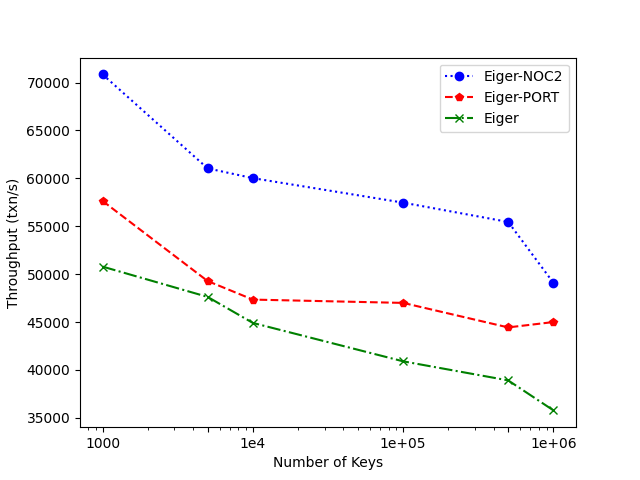
\includegraphics[width=0.8\linewidth]{figure/6-tcc-t.png}
    \caption{Throughput Comparison for Three Different Concurrency Control Algorithms under Different Number of Keys in Causal Consistency Level}
    \label{fig:28}
\end{figure}
\begin{figure}[H]
    \centering
    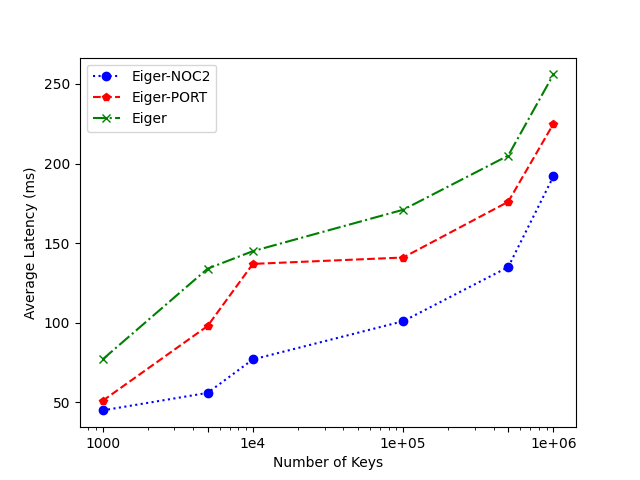
\includegraphics[width=0.8\linewidth]{figure/6-tcc-al.png}
    \caption{Average Latency Comparison for Three Different Concurrency Control Algorithms under Different Number of Keys in Causal Consistency Level}
    \label{fig:29}
\end{figure}
\begin{figure}[H]
    \centering
    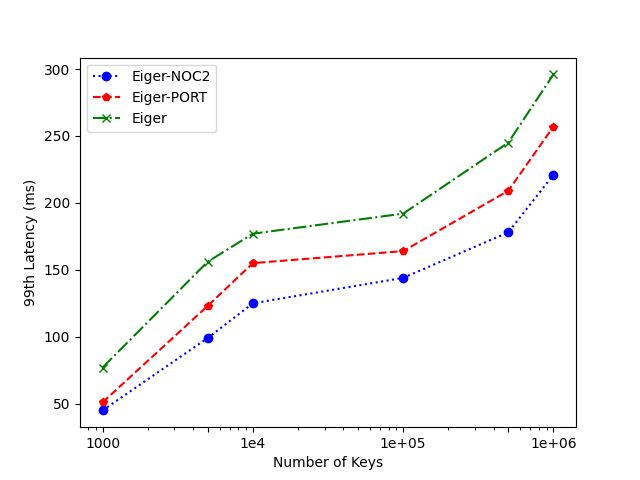
\includegraphics[width=0.8\linewidth]{figure/6-tcc-l.png}
    \caption{99th Latency Comparison for Three Different Concurrency Control Algorithms under Different Number of Keys in Causal Consistency Level}
    \label{fig:30}
\end{figure}


\subsection{Conclusions}
In this chapter, we have conducted extensive experiments to compare algorithms guided by \textbf{NOC-NOC} principles vs. Eiger \cite{lloyd2013stronger}, Eiger-PORT \cite{lu2020performance} and RAMP family algorithms \cite{bailis2016scalable}. Experiment results show that \textbf{NOC-NOC} guided algorithms outperform all other algorithms in these settings. This means that in the current hardware landscape, moving costs from network communication to local computation is always beneficial.  In the future, when the network speed increases significantly, this conclusion may change.